\documentclass[11pt,a4paper]{article}
\usepackage[utf8]{inputenc}
\usepackage{amsmath,amssymb,amsthm}
\usepackage{geometry}
\usepackage{graphicx}
\usepackage{float}
\usepackage[colorlinks=true,linkcolor=black,citecolor=black,urlcolor=black]{hyperref}
\usepackage[
backend=biber,
style=apa,
hyperref=true
]{biblatex}
\addbibresource{references.bib} %Imports bibliography file
\DefineBibliographyStrings{english}{
  bibliography = {References},
}
\geometry{margin=1in}

\title{Application and analysis of SINDy for wave propagation in damaged material}
\author{Carlos Santiago Pineda Morales}
\date{November 13th, 2026}

\begin{document}

\maketitle

\begin{abstract}
Documentation of the methodology used for the application of SINDy and other data driven reduced order model techniques to the wave equation propagating through damaged material, theoretically modeled in 1 and 2 dimensions with partial differential equations, using manufactured solutions to verify the numerical approximations.
\end{abstract}

\section{Wave Equation Model}
The model of the wave equation with a space-dependent wave speed $c(\mathbf{x}) > 0$. In spatial coordinates $\Omega \subset \mathbb{R}^d$ and time $t \in [0, T]$, is given by:
\begin{equation}
    u_{tt}(t, x) - c^2(x) \Delta u(t, x) = f(t, x) \quad \text{in } (0, T) \times \Omega,
\end{equation}
where $u_{tt} = \frac{\partial^2 u}{\partial t^2}$ represents the acceleration of the wave field, and $\Delta u = \frac{\partial^2 u}{\partial x_{1}^2} + ... + \frac{\partial^2 u}{\partial x_{d}^2}$ represents the spatial curvature (Laplacian).

The problem is imposed with homogeneous Dirichlet boundary conditions and the initial conditions, where $u_{0}$ and $u_{1}$ are given functions,

\begin{equation}
    u(0, x) = u_{0}(x), \quad u_{t}(0, x) = u_{1}(x) \quad \text{in } \Omega
\end{equation}

The speed function $c(x)$ can be manipulated such that it has a decrease of speed in a particular point of $\Omega$ representing damaged area in the theoretical material.

\section{1D Wave Equation Model}
Using the suggested approach of manufactured solutions the wave equation was constructed with the following parameters:
\begin{align}
    \text{Spatial Domain:} & \quad \Omega = [0, 1] \\
    \text{Time Horizon:} & \quad t \in [0, 1] \\
    \text{Wave Speed:} & \quad c(x) = 1 + x \\
    \text{Exact Solution:} & \quad u(t, x) = \sin(\pi x) \cos(t) \\
    \text{Initial conditions} & \quad u_{0}(x)= \sin(\pi x), \quad u_{1} = 0
\end{align}

The homogeneous Dirichlet boundary conditions are satisfied since $\sin(\pi x)$ equals zero at the spatial domain $\Omega$ boundaries, that is, $\sin(\pi * 0) = 0$ and $\sin(\pi * 1) = 0$.

Finally, the resulting source term matching the constructed wave equation is,
\begin{align}
    f(t, x) &= (\pi^{2} (1+x)^{2}-1) \sin(\pi x) \cos(t)
\end{align}

\section{Method of Finite Differences}

In the lectures \cite{brunton2022_numerical_diff_1} and \cite{brunton2022_numerical_diff_2} functions $f(t) = \frac{dx}{dt}$ are approximated using numerical differentiation, the derivative formula $\frac{dx}{dt}= \lim_{\Delta t \rightarrow0} \frac{x(t+\Delta t)-x(t)}{\Delta t} \approx\frac{x(t+\Delta t)-x(t)}{\Delta t}$, yielding
\begin{align}
    f(x(t)) \approx \frac{x(t+\Delta t)-x(t)}{\Delta t} \implies x(t +\Delta t) \approx f(x(t)) \Delta t + x(t)
\end{align}

Using the Taylor expansion we can calculate the approximation error,
\begin{align}
    f(t + \Delta t) &= f(t) + \Delta t \, f'(t) + \frac{(\Delta t)^2}{2!} f''(t) + \frac{(\Delta t)^3}{3!} f^{(3)}(t) + \mathcal{O}(\Delta t^4) \\[8pt]
    f(t - \Delta t) &= f(t) - \Delta t \, f'(t) + \frac{(\Delta t)^2}{2!} f''(t) - \frac{(\Delta t)^3}{3!} f^{(3)}(t) + \mathcal{O}(\Delta t^4)
\end{align}

We can approximate each derivative, also second derivatives, in three ways, forward difference (FD), backward difference (BD), and central difference (CD). Note that the central difference is the most accurate approximation, therefore this scheme is used.
\begin{align}
        \frac{df}{dt} \approx \frac{f(t + \Delta t) - f(t - \Delta t)}{2\Delta t} + \mathcal{O}(\Delta t^{2}) \\
         \frac{d^{2}f}{dt^{2}} \approx \frac{f(t + \Delta t) - 2f(t) + f(t - \Delta t)}{\Delta t^{2}} + \mathcal{O}(\Delta t^{2})
\end{align}        

\section{Solving 1D Equation Model with Finite Differences}

The following steps were taken to solve the manufactured equation,

\begin{enumerate}
    \item Discretizations of our space domain and time horizon.
        \begin{align}
            \Delta x = \frac{\Omega_{f} - \Omega_{0}}{N} \quad \implies \quad x_{i}= \Omega_{0} +i\Delta x \\
            \Delta t = \frac{T-0}{M} \quad \implies \quad t_{j}= j\Delta t
        \end{align}
    \item Central difference scheme
        \begin{align}
            u_{tt}(t_{j}, x_{i}) &\approx \frac{u(t_{j+1}, x_{i}) - 2u(t_{j},x_{i}) + u(t_{j-1}, x_{i})}{\Delta t^2} \\
            \Delta u(t_{j},x_{i}) &\approx \frac{u(t_{j}, x_{i+1}) - 2u(t_{j},x_{i}) + u(t_{j}, x_{i-1})}{\Delta x^2}
        \end{align}
    \item Approximating derivatives in the equation using matrix notation $U_{i}^{j} = u(t_{j}, x_{i})$, and $F_{i}^{j} = f(t_{j}, x_{i})$,
        
        \begin{align}
            \frac{1}{\Delta t^2} \left( U_{i}^{j+1} - 2U_{i}^{j} + U_{i}^{j-1}\right) - \frac{c^2(x_i)}{\Delta x^2} \left( U_{i+1}^{j}- 2U_{i}^{j} + U_{i-1}^{j} \right) = F_{i}^{j}
        \end{align}

    \item Solving for the next time step $U_{i}^{j+1}$,
        \begin{align}
            U_{i}^{j+1} = \frac{c^2(x_{i})\Delta t^2}{\Delta x^2}(U_{i+1}^{j} - 2U_{i}^{j}+ U_{i-1}^{j}) + \Delta t^{2}F_{i}^{j} - U_{i}^{j-1} + 2 U_{i}^{j}
        \end{align}

    \item Initializing using Taylor expansion approximation for $u(t_{1},x_i)\equiv u(\Delta t, x_{i})$
        \begin{align}
            u(\Delta t, x_{i}) = u(0, x_{i}) + \Delta t u_{t}(0, x_{i}) + \frac{\Delta t^2}{2}u_{tt}(0, x_i) + \mathcal{O}(\Delta t^3)
        \end{align}
        Using the initial conditions $u_{t}(0, x) = u_{1}(x)$, and $u(0, x_i) = u_{0}(x)$
        \begin{align}
            \implies u_{tt}(0, x_i) \approx \frac{2}{\Delta t^{2}} \left[ u(\Delta t, x_{i}) - u_{0}(x_{i}) - \Delta t u_{1}(x_{i})\right]
        \end{align}
        Using the given wave equation, initial condition $u_{1}(x_{i})=0$, the central difference approximation of $\Delta u(0, x) \equiv \Delta U_{i}^{0}$, and $\Delta t$ representing the first time step taken $j=1$,
        \begin{align}
            U_{i}^{1} = U_{i}^{0} + \frac{\Delta t^2}{2} \left[ c^{2}(x_i)\frac{U_{i+1}^{0} - 2U_{i}^{0}+ U_{i-1}^{0}}{\Delta x^2}+F_{i}^{0} \right]
        \end{align}
    
\end{enumerate}

The comparison between the numerical and exact solutions is shown in Figure one, with an $L^2$ error of just $3.03529e-03$, the numerical approximation is good for applying SINDy and variants.

\begin{figure}[H]
    \centering
    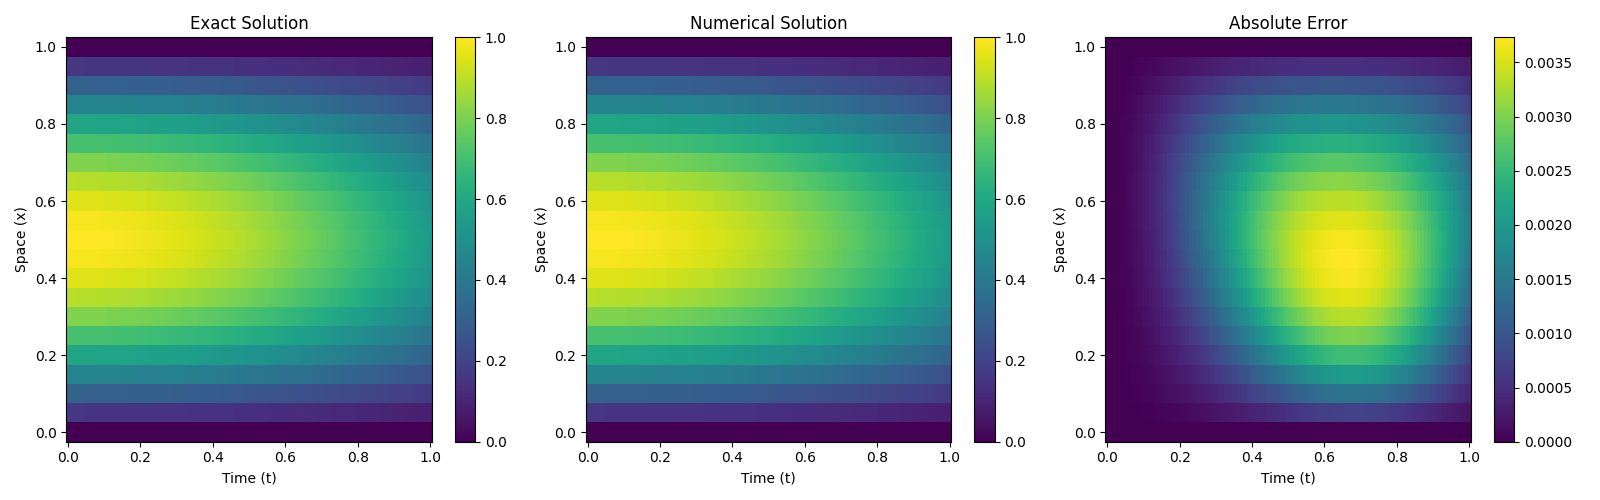
\includegraphics[width=1.0\textwidth]{exact_vs_numerical.png}
    \caption{Comparison between the finite differences numerical and exact solutions for the wave equation.}
\end{figure}

\clearpage
\printbibliography

\end{document}